\uuid{PXTC}
\exo7id{7280}
\titre{exo7 7280}
\auteur{mourougane}
\organisation{exo7}
\datecreate{2021-08-10}
\isIndication{false}
\isCorrection{false}
\chapitre{Géométrie affine euclidienne}
\sousChapitre{Géométrie affine euclidienne du plan}
\module{Géométrie}
\niveau{L2}
\difficulte{}

\contenu{
\texte{

}
\begin{enumerate}
    \item \question{Montrer que pour tout \( \theta \in \Rr\), on~a
\[
\cos(5 \theta) = 16 \cos( \theta)^5 - 20 \cos( \theta)^3 + 5 \cos( \theta).
\]}
    \item \question{En déduire que
$$
\cos\frac{\pi}{5} = \frac{1 + \sqrt{5}}{4} \quad \text{ et } \quad 
\cos\frac{3 \pi}{5} = \frac{1 - \sqrt{5}}{4} $$

$$\sin\frac{ \pi}{10} = \frac{-1 + \sqrt{5}}{4} \quad \text{ et } \quad 
\sin\frac{3 \pi}{10} = \frac{1 + \sqrt{5}}{4}.
$$

On vérifiera que
\[
16 X^5 - 20 X^3 + 5 X + 1 = (X + 1) (4 X^2 - 2 X - 1)^2.
\]}
    \item \question{Quelle est la longueur des côtés d'un pentagone régulier inscrit 
dans un cercle de rayon \(1\)? celle d'un décagone régulier?}
    \item \question{On considère la construction suivante:

\begin{center}
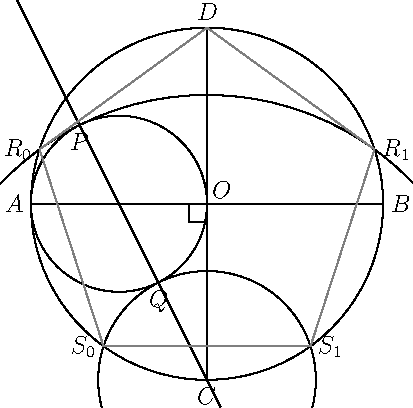
\includegraphics[scale=1]{images/img-mour-032}
\end{center}

% [[figure asymptote]]

%\begin{center}
%\medskip
%\begin{asy}
%size(7cm, 0);
%point O = (0, 0); label("\(O\)", O, NE);
%circle C0 = circle(O, 1); draw(C0);
%point A = (-1, 0); label("\(A\)", A, W);
%point B = (1, 0); label("\(B\)", B, E);
%draw(A--B);
%circle C1 = circle(A, O); draw(C1);
%point C = (0, -1); label("\(C\)", C, S);
%point D = (0, 1); label("\(D\)", D, N);
%draw(C--D);
%perpendicularmark(line(O, A), line(O, C));
%line D0 = line(0.5*A + 0.5*O, C);
%draw(D0);
%point[] PQ = intersectionpoints(C1, D0);
%point P = PQ[1]; label("\(P\)", P, S);
%point Q = PQ[0]; label("\(Q\)", Q, S);
%circle C2 = circle(C, abs(P-C));
%clipdraw(C2);
%circle C3 = circle(C, abs(Q-C));
%clipdraw(C3);
%point[] R = intersectionpoints(C0, C2);
%point[] T = intersectionpoints(C0, C3);
%label("\(R_0\)", R[0], W);
%label("\(R_1\)", R[1], E);
%label("\(S_0\)", T[0], W);
%label("\(S_1\)", T[1], E);
%draw(D -- R[0] -- T[0] -- T[1] -- R[1] -- cycle, gray);
%\end{asy}
%\end{center}


Les segments \([AB]\) et \([CD]\) sont deux diamètres orthogonaux d'un 
cercle \(\mathcal{C}\) de centre \(O\). Notons \(\mathcal{C}_1\) le cercle 
de diamètre \([AO]\), et \(P\) et \(Q\) les points d'intersection du 
cercle \(\mathcal{C}_1\) et de la droite passant par \(C\) et par le 
centre de \(\mathcal{C}_1\). Soient \(R_0\) et \(R_1\) les points 
d'intersection de \(\mathcal{C}\) et du cercle de centre \(C\) passant 
par \(P\), et soient \(S_0\) et \(S_1\) les points d'intersection 
de \(\mathcal{C}\) et du cercle de centre \(C\) passant par \(Q\). 
Calculer les longueurs \(CP\) et \(CQ\).}
    \item \question{En déduire la mesure des angles \(\widehat{COR_0}\) 
et \(\widehat{COS_0}\).}
    \item \question{En déduire que les points \(D R_0 S_0 S_1 R_1\) forment un pentagone 
régulier.}
\end{enumerate}
}
